
\chapter{Regular collapsing and applications}\label{chap7}

\section{Regular collapsing}\label{chap7-sec7.1}\pageoriginale
Let $\mathscr{S}$ be a simplicial presentation. We say that $\sigma \in \mathscr{S}$ is an {\em outer edge} of $\mathscr{S}$, if there is a $\Delta\in \mathscr{S}$, such that if $\sigma\leq \rho$, $\rho\in\mathscr{S}$, then $\rho\leq \Delta$, and $\dim \Delta >\dim \sigma$. In this case $\Delta$ is uniquely fixed by $\sigma$, and is of the form $\Delta =\sigma\tau$, $\tau\neq \emptyset$. The elements of $\mathscr{S}$ having $\sigma$ as a face are exactly of the form $\sigma\tau'$, $\tau'\leq \tau$. The remaining faces of $\Delta$ are of the form $\sigma'\tau'$, $\sigma'<\sigma$, $\tau'\leq \tau$; in otherwords they consist of $\{\p \sigma\}\ast\{\overline{\tau}\}$. Thus 
$$
\mathscr{S}'=\mathscr{S}-\{\overline{\Delta}\}\cup [\{\p \sigma\}\ast\{\overline{\tau}\}]
$$
is a subpresentation of $\mathscr{S}$, and 
\begin{gather*}
|\mathscr{S}|=|\mathscr{S}'|\cup \overline{\Delta}\\
|\mathscr{S}'|\cap \overline{\Delta}=\p \sigma\ast\overline{\tau}
\end{gather*}

Let $\dim =\Delta=n$. Then, we say that $\mathscr{S}'$ is obtained from $\mathscr{S}$ by an {\em elementary regular collapse} $(n)$ with outer edge $\sigma$ and {\em major simplex} $\Delta$.

If $\mathscr{S}=\mathscr{S}_{1},\ldots,\mathscr{S}_{k}=\mathscr{Z}$, and $\mathscr{S}_{i+1}$ is obtained from $\mathscr{S}_{i}$ by an elementary regular collapse $(n)$, we say that $\mathscr{S}$ {\em regularly collapses} $(n)$ to $\mathscr{Z}$. 

The elements of the theory of regular collapsing can be approached from the point of view of ``steller subdivisions'' (cf.\@ Section 13 of ``simplicial spaces, nuclei and $m$-groups'' or the first few pages of Zeeman's ``unknotting spheres'', Annals of Mathematics, 72, (1960) 350-361), but for the sake of novelty we shall to something else. 

\subsection{Recalling Notations.}\label{chap7-sec7.1.1}\pageoriginale
$\sigma$, $\tau,\ldots$ usually denote open
simplexes. $\overline{\sigma}$, $\overline{\tau},\ldots$ denote their
closures {\small (closed simplexes)}, and $\p \sigma$, $\p \tau,\ldots$ their boundaries. The simplicial presentation of $\overline{\sigma}$ consisting of $\sigma$ and its faces in denoted by $\{\overline{\sigma}\}$, and that of $\p \sigma$ consisting of faces of $\sigma$ by $\{\p \sigma\}$ (see \ref{chap4-sec4.1}). $\sigma\tau$ stands for the join of the two open simplexes $\sigma$ and $\tau$, when the join is defined. If $\sigma$ is a $0$-simplex and $x$ is the unique point of $\sigma$, we will write $\{x\}\tau$ for $\sigma\tau$. On the other hand the join of two polyhedra $P$ and $Q$ when it is defined is denoted by $P\ast Q$. Similarly the join of two simplicial presentations $\mathscr{P}$ and $\mathcal{Q}$ when it is defined is denoted by $\mathscr{P}\ast \mathcal{Q}$. For example if $\sigma\tau$ is defined, then $\{\p \sigma\}\ast\{\overline{\tau}\}$ is the canonical simplicial presentation of the polyhedron $\p \sigma\ast\overline{\tau}$. If $P$ is a polyhedron consisting of a single 
point $x$, we will sometimes write $x\ast Q$ instead of $P\ast Q$. With this notation $\overline{\{x\}\sigma}$ and $x\ast \overline{\sigma}$ are the same.

Let $\Delta$ be an $(n-1)$-simplex, $I=[0,1]$, and let $\mathscr{S}$ be a simplicial presentation of $\overline{\Delta}\times I$ such that the projection $p:\overline{\Delta}\times I\to \overline{\Delta}$ is simplicial with reference to $\mathscr{S}$ and $\{\overline{\Delta}\}$.

The $n$-simplexes of $\mathscr{S}$ can be ordered as follows: $\Gamma_{1},\ldots,\Gamma_{k}$, so that if $x\in\Delta$, $x\times I$ intersects the $\Gamma_{i}$'s in order. That is $\Delta \times 0$ is a face of $\Gamma_{1}$, $\Gamma_{1}$ has another face $\Delta_{1}$ which maps onto $\Delta$, $\Delta_{1}$ is a face of $\Gamma_{2},\ldots,\Delta_{i-1}$ is a face of $\Gamma_{i}$, but $\Gamma_{i}$ has another face that maps onto $\Delta$, call it $\Delta_{i}$ and so on. We start with $\Delta_{0}=\Delta\times 0$ and end up with $\Delta_{k}=\Delta\times 1$.

Let\pageoriginale us write $\Delta=\sigma\tau$ in some way. Let $T=\overline{\Delta}\times 0\cup (\p \sigma\ast\overline{\tau})\times I$. (If $\sigma=\emptyset$, $T$ should be taken to be just $\overline{\Delta}\times 0$). Then there is a subpresentation $\mathscr{Z}$ of $\mathscr{S}$ which covers $T$.

\setcounter{lemma}{1}
\begin{lemma}\label{chap7-lem7.1.2}
(With the above hypotheses and notation) $\mathscr{S}$ regularly collapses $(n)$ to $\mathscr{Z}$.
\end{lemma}

\begin{proof}
We in fact show that there is a sequence of regular collapses with major simplexes $\Gamma_{k},\ldots,\Gamma_{1}$. We must then define
$$
\mathscr{S}_{i}=\mathscr{Z}\cup \{\overline{\Gamma}_{1}\}\cup \ldots\cup \{\overline{\Gamma}_{i}\}
$$
and find some outer edge lying on $\overline{\Gamma}_{i}$, so that the corresponding regular collapse results in $\mathscr{S}_{i-1}$.

Now $\Gamma_{i}$ is an $n$-simplex and its projection $\Delta$ is an $(n-1)$-simplex, therefore there are two vertices $v_{1}$ and $v_{2}$ of $\Gamma_{i}$ (choose $v_{1}$, $v_{2}$ so that the $I$-co-ordinate of $v_{1}$ is $<$ the $I$-co-ordinate of $v_{2}$) which map into one vertex $v$ of $\Delta$. Now $\Delta=\sigma\tau$ and so $v$ is a vertex of either $\sigma$ or $\tau$.

\medskip
\noindent
{\bf Case 1:}~ $v$ is a vertex of $\sigma$. Write $\sigma=\{v\}\sigma'$. Let $\overline{\sigma}'$ and $\overline{\tau}$ be the faces of $\Gamma_{i}$ lying over $\sigma'$ and $\tau$. Then
$$
\Gamma_{i}=\{v_{1}\}\{v_{2}\}\tilde{\sigma}'\tilde{\tau}
$$
and the two faces of $\Gamma_{i}$ which are mapped onto $\Delta$ are
\begin{align*}
& \{v_{1}\}\tilde{\sigma}'\tilde{\tau}=\Delta_{i-1}\\
\text{and}\qquad & \{v_{2}\}\tilde{\sigma}'\tilde{\tau}=\Delta_{i}.
\end{align*}

Define $\sigma_{i}=\{v_{2}\}\tilde{\sigma}'$, $\tau_{i}=\{v_{1}\}\tilde{\tau}$. It\pageoriginale is claimed that if we take $\sigma_{i}$ as an outer edge then the result of the elementary regular collapse with major simplex $\Gamma_{i}$ is $\mathscr{S}_{i-1}$. 
\begin{figure}[H]
\centering
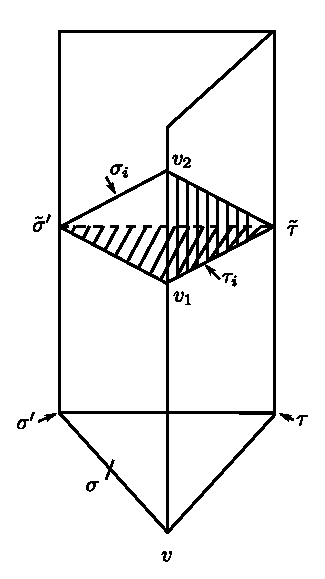
\includegraphics{figure/fig19.eps}
\end{figure}
\end{proof}

$\sigma_{i}$ cannot be in $\mathscr{Z}$; because the only $(\dim\sigma)$-simplex in $\sigma\times I$ which is in $\mathscr{Z}$ is $\sigma$, and $\sigma_{i}\neq \sigma$ since $v_{2}$ is a vertex of $\sigma_{i}$. Also $\Gamma_{i}$ is the only simplex among $\Gamma_{1},\ldots,\Gamma_{i}$ which contains $v_{2}$ as a vertex. Hence if $\sigma_{i}\leq \rho$, $\rho\in \mathscr{S}_{i}$, then $\rho\leq \Gamma_{i}$. 

We then have to show that $\overline{\Gamma}_{i}\cap \mathscr{S}_{i-1}=\p \sigma_{i}\ast\tau_{i}$
\begin{align*}
\p \sigma_{i}\ast\overline{\tau}_{i} &= \p (\{v_{2}\}\tilde{\sigma}')\ast (\overline{\{v_{1}\}\tilde{\tau}})\\
&= (\overline{\tilde{\sigma}'\{v_{1}\}\tilde{\tau}})\cup (v_{2}\ast\p \tilde{\sigma}'\ast \overline{\{v_{1}\}\tilde{\tau}}).
\end{align*}

The first term here is $\overline{\Delta}_{i-1}$, which is where $\overline{\Gamma}_{i}$ intersects $\overline{\Gamma}_{1}\cup\ldots\cup \overline{\Gamma}_{i-1}$. The\pageoriginale second term written slightly differently is $[v_{1}v_{2}]\ast \p \tilde{\sigma}'\ast\overline{\tilde{\tau}}$ to which we may add a part of the first term namely $(\overline{\tilde{\sigma}'\tilde{\tau}})$ to obtain all faces of $\Gamma_{i}$ which map to 
\begin{align*}
\p \sigma\ast\overline{\tau} &= \p(\{v\}\sigma^{1})\ast\overline{\tau}\\
&=(\overline{\sigma}'\ast\overline{\tau})\cup [\p \sigma'\ast\overline{\tau}\ast v]
\end{align*}

In other words, this is $\overline{\Gamma}_{i}\cap [(\p \sigma\ast\overline{\tau})\times I]$.

This shows that
$$
\overline{\Gamma}_{i}\cap |\mathscr{S}_{i-1}|=\p \sigma_{i}\ast\overline{\tau}_{i};
$$
and so $\mathscr{S}_{i}$ to $\mathscr{S}_{i-1}$ is an elementary regular collapse with outer edge $\sigma_{i}$ and major simplex $\Gamma_{i}$.

\noindent
{\bf Case 2:}~ $v$ is a vertex of $\tau$. Wrtie $\tau=v\tau'$, define $\tilde{\sigma}$, $\tilde{\sigma}'$ to be faces of $\Gamma_{i}$ lying over $\sigma$ and $\tau'$. In this case 
$$
\Gamma_{i}=\{v_{1}\}\{v_{2}\}\tilde{\sigma}\tilde{\tau}'
$$
and the two faces of $\Gamma_{i}$ which are mapped on $\Delta$ are 
\begin{align*}
& \{v_{1}\}\tilde{\sigma}\tilde{\sigma}'=\Delta_{i-1}\\
\text{and}\qquad & \{v_{2}\}\tilde{\sigma}\tilde{\tau}'=\Delta_{i}.
\end{align*}

We now define
\begin{align*}
\sigma_{i} &=\{v_{2}\}\tilde{\sigma}\\
\tau_{i} &= \{v_{1}\}\tilde{\tau}'
\end{align*}
and make computations as before.
\begin{align*}
& \p \sigma_{i}\ast\overline{\tau}_{i}\\
&= (\overline{\tilde{\sigma}}\ast\overline{\{v_{1}\}\tilde{\tau}'})\cup (v_{2}\ast\p \tilde{\sigma}\ast\overline{\{v_{1}\}\tilde{\tau}'})\\
&= \overline{\Delta}_{i-1}\cup \p \tilde{\sigma}\ast[v_{1}v_{2}]\ast \overline{\tilde{\tau}'}
\end{align*}
and\pageoriginale $\p \tilde{\sigma}\ast [v_{1}v_{2}]\ast \overline{\tilde{\tau}'}=\overline{\Gamma}_{i}\cap [(\p \sigma\ast \overline{\tau})\times I]$
\begin{figure}[H]
\centering
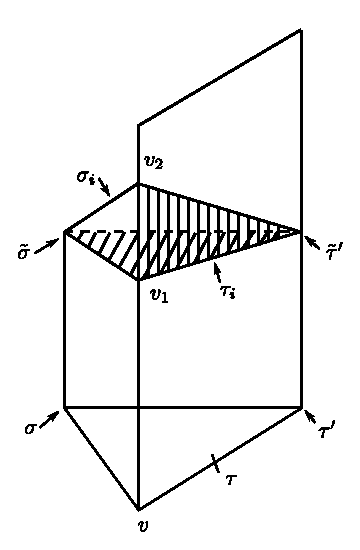
\includegraphics{figure/fig20.eps}
\end{figure}

And this shows that if we perform an elementary regular collapse $(n)$ on $\mathscr{S}_{i}$ with outer edge $\sigma_{i}$ and major simplex $\Gamma_{i}$, we get $\mathscr{S}_{i-1}$.

Hence $\mathscr{S}$ regularly collapses $(n)$ to $\mathscr{Z}$.

Define $I^{1}=I$, $I^{k}=I^{k-1}\times I$, $T_{1}=0\subset I'$, and $T_{k}=(I^{k-1}\times 0)\cup (T_{k-1}\times I)\subset I^{k}$.

It is easy to see that $T_{k}$ is a $(k-1)$-cell in $\p I^{k}$, and is the set of points of $I^{k}$ at least one co-ordinate of which is zero.

Let\pageoriginale $\alpha_{k}:I^{k}=I^{k-1}\times I\to I^{k-1}$ be the projection. 

\begin{lemma}\label{chap7-lem7.1.3}
Let $\mathscr{S}_{n}$, $\mathscr{S}_{n-1},\ldots,\mathscr{S}_{1}$ be simplicial presentations of $I^{n}$, $I^{n-1},\ldots,I^{1}$ with respect to which all the maps $\alpha_{n},\ldots,\alpha_{2}$, are simplicial. Then there exist subpresentations $\mathscr{Z}_{n}$, $\mathscr{Z}_{n-1},\ldots,\mathscr{Z}_{1}$ covering $T_{n}$, $T_{n-1},\ldots,T_{1}$ respectively, and such that $\mathscr{S}_{i}$ regularly collapses (i) to $\mathscr{Z}_{i}$ for all $i$. 
\end{lemma}

\begin{proof}
The proof is by induction. It is easily verified that $\mathscr{S}_{1}$ collapses (1) to $\mathscr{Z}_{1}$.

So, inductively, we know that $\mathscr{S}_{i}$ collapses (i) to $\mathscr{Z}_{i}$, for $i\leq n-1$. Now $\mathscr{Z}_{n}$ is just the subpresentation of $\mathscr{S}_{n}$ covering $I^{n-1}\times 0\cup |\mathscr{Z}_{n-1}|\times I=T_{n}$.

Let the collapsing of $\mathscr{S}_{n-1}$ to $\mathscr{Z}_{n-1}$ occur along the major simplexes $\Delta_{1},\ldots,\Delta_{k}$. Then we define
$$
\mathfrak{a}_{i}=\mathscr{Z}_{n-1}\cup \{\overline{\Delta}_{i}\}\ldots \{\overline{\Delta}_{k}\}
$$
and write $\Delta_{i}=\sigma_{i}\tau_{i}$, where $\sigma_{i}$ is the outer edge of the regular collapse $(n-1)$ from $\mathfrak{a}_{i}$ to $\mathfrak{a}_{i+1}$. Then $\overline{\Delta}_{i}\cap |\mathfrak{a}_{i+1}|=\p \sigma_{i}\ast \overline{\tau}_{i}$.

Define $\mathscr{B}_{i}=$ the subpresentation of $\mathscr{S}_{n}$
covering $I^{n-1}\times 0$ plus
$\alpha^{-1}_{n}\break(|\mathfrak{a}_{i}|)$. Thus
$\mathscr{B}_{1}=\mathscr{S}_{n}$ and
$\mathscr{B}_{k+1}=\mathscr{Z}_{n}$. 

We will show that $\mathscr{B}_{i}$ regularly collapses $(n)$ to $\mathscr{B}_{i+1}$, stringing these together, then $\mathscr{S}_{n}$ regularly collapses $(n)$ to $\mathscr{Z}_{n}$.

To\pageoriginale show that $\mathscr{B}_{i}$ regularly collapses $(n)$ to $\mathscr{B}_{i+1}$ it is enough to look at the part of $\mathscr{B}_{i}$ covering $\alpha^{-1}_{n}(\overline{\Delta}_{i})$ i.e.\@ $\overline{\Delta}_{i}\times I$. $\overline{\Delta}_{i}\times I\cap |\mathscr{B}_{i+1}|=\overline{\Delta}_{i}\times 0\cup [(\p \sigma_{i}\ast \overline{\tau}_{i})\times I]$ and $\alpha_{n}|\overline{\Delta}_{i}\times I$ is just the projection $\overline{\Delta}_{i}\times I\to \overline{\Delta}_{i}$ which is simplicial with reference to the subpresentation of $\mathscr{S}_{n}$ covering $\overline{\Delta}_{i}\times I$ and $\{\overline{\Delta}_{i}\}$. And our lemma \ref{chap7-lem7.1.2} is especially tailored for this situation.
\end{proof}

\setcounter{proposition}{3}
\begin{theorem}\label{chap7-thm7.1.4}
Let $A$ be a $n$-cell, $B$ an $n$-cell in $A$, and $\mathscr{P}$ a regular presentation of $A$. Then there is a simplicial presentation $\mathscr{S}$ refining $\mathscr{P}$, with a subpresentation $\mathscr{Z}$ covering $B$, such that $\mathscr{S}$ regularly collapses $(n)$ to $\mathscr{Z}$.
\end{theorem}

\begin{proof}
There is a polyhedral equivalence $h:A\to I^{n}$, with $h(B)=T^{n}$. Then $h$ is simplicial with reference to some $\mathscr{P}_{1}$ and $\mathcal{Q}$, where $\mathscr{P}_{\alpha_{n}}$ can be assumed to refine $\mathcal{Q}$. The diagram
$$
I^{n}\xrightarrow{\alpha_{n}}I^{n-1}\to \ldots \xrightarrow{\alpha_{2}}I'
$$
can be triangulated by simplicial presentations $\mathscr{S}_{n},\ldots,\mathscr{S}_{1}$, where $\mathscr{S}_{n}$ can be assumed to refine $\mathcal{Q}$. By \ref{chap7-lem7.1.3}, $\mathscr{S}_{n}$ regularly collapses $(n)$ to $\mathscr{Z}_{n}$, the subpresentation of $\mathscr{S}_{n}$ covering $T_{n}$. Therefore the isomorphic presentation $h^{-1}(\mathscr{S}_{n})=\mathscr{S}$ collapses regularly $(n)$ to $h^{-1}(\mathscr{Z}_{n})=\mathscr{Z}$.
\end{proof}

Suppose that $\mathscr{S}$ is a simplicial presentation of an $n$-cell $A$, regularly collapsing $(n)$ to $\mathscr{Z}$, $(|\mathscr{Z}|)=B$, an $(n-1)$-cell in $\p A$. Let the intermediate stages be
$$
\mathscr{S}=\mathscr{S}_{1},\ldots,\mathscr{S}_{k}=\mathscr{Z},
$$
where\pageoriginale is obtained from $\mathscr{S}_{i}$ by a regular collapse $(n)$ at outer edge $\sigma_{i}$ and major simplex $\Delta_{i}=\sigma_{i}\tau_{i}$.
\begin{quote}
We define the upper boundary of $\mathscr{S}_{i}$ as follows:

upper boundary of $\mathscr{S}_{1}=\p (|\mathscr{S}_{1}|)$-interior $(|\mathscr{Z}|)$

upper boundary of $\mathscr{S}_{i+1}$

= (upper boundary of $\mathscr{S}_{i} - \overline{\sigma}_{i}\ast\p\tau_{i})\cup \p \sigma_{i}\ast \overline{\tau}_{i}$.
\end{quote}

It can be alternatively defined as follows: Upper boundary of $\mathscr{S}_{i}=$ unions of closures of $(n-1)$-cells $E$ of $\mathscr{S}_{i}$, such that if $E\not\in \mathscr{Z}$, $E$ is the face of exactly one $n$-simplex of $\mathscr{S}_{i}$ and if $E\in\mathscr{Z}$ then $E$ is the face of no $n$-simplex of $\mathscr{S}_{i}$.

Now we would like to assert that

\setcounter{subsection}{4}
\subsection{}\label{chap7-sec7.1.5}
\begin{itemize}
\item[(a)] The upper boundary of $\mathscr{S}_{i}$ is an $(n-1)$-cell, with constant boundary $\p(|\mathscr{Z}|)$. The upper boundary of the last stage is $|\mathscr{Z}|$.

\item[(b)] $\overline{\Delta}_{i}$ intersects the upper boundary of precisely along $\overline{\sigma}_{i}\ast\p\tau_{i}$. In particular $\tau_{i}$ cannot be in the upper boundary of $\mathscr{S}_{i}$ for any $i$, hence can never be in $\p |\mathscr{Z}|$.
\end{itemize}

If in \ref{chap7-lem7.1.3}, in each column we do the collapsing as described in \ref{chap7-lem7.1.2}, the above assertions can be verified in a straight forward manner, by using similar properties of $\mathscr{S}_{n-1}$ and an analysis of the individual steps in \ref{chap7-lem7.1.2}. The general case seems to be more cumbersome (A proof is given in the appendix). But the special case is enough for our purposes, namely for the next theorem, the main result of this chapter.

First using \ref{chap7-sec7.1.5}, we define a polyhedral equivalence $\varphi_{i}$ from the upper boundary of $\mathscr{S}_{i}$ to the upper boundary of $\mathscr{S}_{i+1}$ by $\varphi_{i}=$\pageoriginale identity outside $\overline{\sigma}_{i}\ast \p \tau_{i}$, and on $\overline{\sigma}_{i}\ast\p \tau_{i}$, it is the join of the identity map $\p \sigma_{i}\ast\p \tau_{i}$ to the map of centre of $\sigma_{i}$ to the centre of $\tau_{i}$.

Thus from $\overline{\p|\mathscr{S}|-|\mathscr{Z}|}$ to $|\mathscr{Z}|$, we reach by simplicial moves, never disturbing the boundary of $|\mathscr{Z}|$.

\setcounter{proposition}{5}
\begin{theorem}\label{chap7-thm7.1.6}
Let $D$ be a $(k+1)$-cell contained in the interior of an $n$-cell $\Delta$. Let $\p D=E_{1}\cup E_{2}$, $E_{1}$ and $E_{2}$ two $k$-cells, $\p E_{1}=\p E_{2}$; let $X\subset \Delta$ be a polyhedron such that $X\cap D\subset \p E_{1}$. Then there is an isotopy of $\Delta$, fixed on $X\cup \p \Delta$, taking $E_{1}$ onto $E_{2}$.
\end{theorem}

\medskip

\begin{proof}
~\phantom{a}

\begin{figure}[H]
\centering
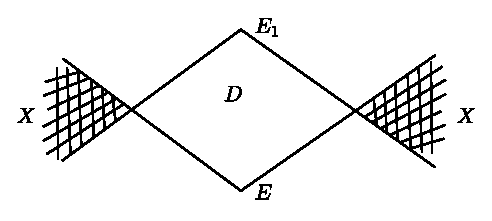
\includegraphics{figure/fig21.eps}
\end{figure}

Consider $\Delta$ to be a standard $n$-cell, we can suppose that $\p \Delta \subset X$, and triangulate the whole picture, so that there are subpresentations covering $D$, $X$. Refine the subpresentation covering $D$, to $\mathscr{S}$, which regularly collapses $(K+1)$ to $\mathscr{Z}$ which covers $E_{2}$. Extend $\mathscr{S}$ to the whole of $\Delta$, to say $\mathscr{P}$. Let the intermediate stages of the collapsing be
$$
\mathscr{S}=\mathscr{S}_{1},\ldots,\mathscr{S}_{p}=\mathscr{Z},
$$
$\mathscr{S}_{i+1}$ obtained from $\mathscr{S}_{i}$ by an elementary regular collapse $(k+1)$ at\pageoriginale out edge $\sigma_{i}$ and major simplex $\Gamma_{i}=\sigma_{i}\tau_{i}$.

We will find an isotopy taking the upper boundary of $\mathscr{S}_{i}$ to the upper boundary of $\mathscr{S}_{i+1}$, and fixed except in a certain $n$-cell to be described.

$\Gamma_{i}$ is a $(k+1)$-simplex contained in the complement of $X$, which is also covered by a subpresentation of $\mathscr{P}$. So if take $|\lambda_{\mathscr{P}}\Gamma_{i}|=\sum$, say, $\sum\ast \overline{\Gamma}_{i}\subset \Delta$, and $(\sum\ast\overline{\Gamma}_{i})\cap X=\overline{\Gamma}_{i}\cap X$. Now $\overline{\Gamma}_{i}\cap X$ must be contained in $\p \sigma_{i}\ast \p \tau_{i}$, for this is the only part of $\overline{\Gamma}_{i}$ which could contain points in $\p E_{i}$. Let $s$ and $t$ be the centres of $\sigma_{i}$ and $\tau_{i}$, the line segment $[s,t]$ can be prolonged a little bit (here we use the fact that $\Delta$ is standard) to $v$ and $w$ in $\Delta$, so that
\begin{align*}
& \left([v,w]\ast(\p \sigma_{i}\ast\p\tau_{i})\ast\sum\right)\cap X\subset \p \sigma_{i}\ast\p \tau_{i}\\
& \left([v,w]\ast (\p \sigma_{i}\ast \p \tau_{i})\ast \sum\right)\cap\text{~ upper boundary}
\end{align*}
of $\mathscr{S}_{i}\subset \p \sigma_{i}\ast \p \tau_{i}$. (here we use the fact that if $L\cap (\overline{\sigma}\ast K)\subset L\cap K$, where $\sigma$ is a simplex and $K$, $L$ are polyhedra, then there is a stretching $\sigma'$ of $\sigma$ i.e.\@ containing $\overline{\sigma}$ such that $L\cap (\overline{\sigma}'\ast K)\subset K\cap L$). Thus we have in order $\{v,s,t,w\}$ and there is a polyhedral equivalence $f$ of $[v,w]$, taking $v$ to $v$, $s$ to $t$ and $w$ to $w$. Join $f$ to the identity on $\p \sigma_{i}\ast \p \tau_{i}\ast\sum$ and extend by identity outside of $[v,w]\ast \p \sigma_{i}\ast \p \tau_{i}\ast\sum$; call it $h_{i}$. Now $h_{i}$ is the result of a nice isotopy and takes the upper boundary of $\mathscr{S}_{i}$ to the upper boundary of $\mathscr{S}_{i+1}$.

The\pageoriginale composition of the $h_{i}$, will then take the upper boundary of $\mathscr{S}_{1}=E_{1}$ to the upper boundary of $\mathscr{S}_{p}=E_{2}$.
\end{proof}

\begin{remark}\label{chap7-rem7.1.7}
In theorem \ref{chap7-thm7.1.6}, $\Delta$ can be replaced by any PL-manifold. Of course $D$ should be in the interior.
\end{remark}

\begin{ex}\label{chap7-ex7.1.8}
If $N$ and $M$ are two PL-manifolds and $f:N\times I\to \text{int\,}M$ an imbedding, show that there is an isotopy of $M$ fixing $\p M$ and carrying $f(N\times 0)$ to $f(N\times 1\cup \p N\times I)$. If $X$ is a polyhedron in $M$, and $X\cap f(N\times I)\subset \p f(N\times 0)$, the isotopy can be chosen to leave $X$ fixed.
\end{ex}

\section{Applications}\label{chap7-sec7.2}

\begin{definition}\label{chap7-defi7.2.1}
Let $S$ be an $n$-sphere, and $\sum$ a $k$-sphere in $S$. The pair $(S,\sum)$ is said to be {\em unknotted} if $(S,\sum)$ is polyhedrally equivalent to $(X\ast \sum,\sum)$ for some $X$.

$X$ must of course be an $(n-k-1)$-sphere. Clearly a pair equivalent to an unknotted pair is again unknotted.
\end{definition}

\begin{proposition}\label{chap7-prop7.2.2}
Let $S$ be an $n$-sphere, and $\sum$ a $k$-sphere in $S$. If there exists an $(n-k-1)$-cell $D$ in $S$ such that $D\ast \sum \subset S$, then $(S,\sum)$ is unknotted.
\end{proposition}

\begin{proof}
$D\ast \sum$ is an $n$-cell, and so the closure of $S-D\ast\sum$, say $\Delta$, is again an $n$-cell and $\p \Delta =\p (D\ast\sum)=\p D\ast \sum$. Then $S$ is polyhedrally equivalent to a suspension of $\p D\ast \sum$, hence $(S,\sum)$ is equivalent $(X\ast \sum,\sum)$ where $X$ is a suspension of $\p D$.
\end{proof}

\begin{corollary}\label{chap7-coro7.2.3}
If $\mathscr{P}$ is a regular presentation of an $n$-sphere $S$, and $A$ a $(k+1)$-cell in $\mathscr{P}$, then $(S,\p A)$ is unknotted.
\end{corollary}

\begin{proof}
Take\pageoriginale $D=|\delta_{\mathscr{P}}A|$ (with respect to some centering of $\mathscr{P}$) in \ref{chap7-prop7.2.2}.
\end{proof}

\begin{proposition}\label{chap7-prop7.2.4}
If a $k$-sphere $\sum$ bounds a $(k+1)$-cell $D$ contained in the interior of a PL-manifold $M$, then there is an isotopy of $M$ taking $\sum$ onto the boundary of a $(k+1)$-cell of some regular presentation of $M$.
\end{proposition}

\begin{proof}
Take a regular presentation $\mathscr{P}$ of $M$ in which $D$ is covered by a full subpresentation $\mathcal{Q}$. Consider a $k$-cell $E$ of $\mathcal{Q}$ in $\p D$ and the $(k+1)$-cell, say $A$ of $\mathcal{Q}$, which contains it in its boundary. Let $\overline{\p A-E=E_{1}}$ and $\overline{\p D-E}=E_{2}$ and $\overline{D-A}=D'$. Then $D'$ is a $(k+1)$-cell with boundary $E_{1}\cup E_{2}$ and $E$ intersect $D'$ in $\p E_{1}=\p E_{2}$. Hence by theorem \ref{chap7-thm7.1.6}, there is an isotopy of $M$ taking $E_{2}$ onto $E_{1}$ and fixing $E$. Thus $\p D$ will be moved onto $\p A$.
\begin{figure}[H]
\centering
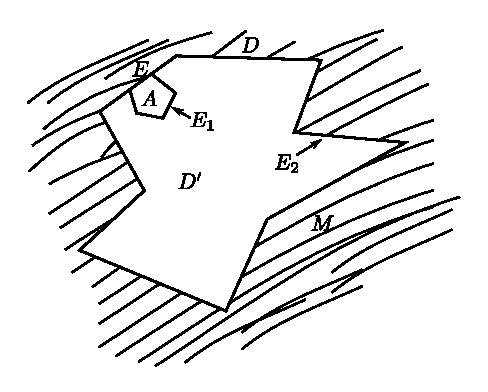
\includegraphics{figure/fig22.eps}
\end{figure}
\end{proof}

\begin{corollary}\label{chap7-coro7.2.5}
Let $S$ be an $n$-sphere, and $\sum$ a $k$-sphere in $S$. $(S,\sum)$ is unknotted if and only if $\sum$ bounds a $(k+1)$-cell in $S$.
\end{corollary}

\begin{proof}
The necessity is clear. Sufficiency follows from \ref{chap7-prop7.2.4} and \ref{chap7-coro7.2.3}. 
\end{proof}

Motivated by \ref{chap7-prop7.2.4}, we define a $k$-sphere $\sum$ in the {\em interior} of a PL-manifold $M$ to be {\em unknotted} if it bounds a $(k+1)$-cell\pageoriginale in (the interior of) $M$. From \ref{chap7-prop7.2.4} it is clear that 

\setcounter{subsection}{5}
\subsection{}\label{chap7-sec7.2.6}
If $A$ is a $(k+1)$-cell of some regular presentation of $M$, and $\overline{A}\subset \text{int\,}M$, then $\p A$ is unknotted. If $\sum_{1}$ and $\sum_{2}$ are two unknotted spheres in the same component of $M$, there is an isotopy of $M$ which takes $\sum_{1}$ onto $\sum_{2}$ keeping $M$ fixed.

\setcounter{proposition}{6}
\begin{definition}\label{chap7-defi7.2.7}
If $D$ is an $n$-cell and $E$ a $k$-cell in $D$, with $\p D\subset \p E$, $(D,E)$ is said to be {\em unknotted if} $(D,E)$ is polyhedrally equivalent to $(X\ast E,E)$ for some $X$.
\end{definition}

Since $E$ is not completely contained in $\p D$, such an $X$ must be an $(n-k-1)$-sphere.

And we define a cell $E$ in the {\em interior} of a PL $n$-manifold $M$ to be {\em unknotted}, if there is an $n$-cell $D$ in $M$ containing $E$ such that $(D,E)$ is unknotted. A cell which is the closure of an open convex cell of some regular presentation of $M$ is clearly unknotted. Given any two unknotted cells $D_{1}$ and $D_{2}$ of the same dimension in $M$, there is an isotopy of $M$ leaving $\p M$ fixed and taking $D_{1}$ onto $D_{2}$. Given two unknotted $k$-cells $D_{1}$ and $D_{2}$ in a PL $n$-manifold $M$, $k<n$, $D_{1}\cap D_{2}=\emptyset$, then there is a $n$-cell $A$ containing $D_{1}$ and $D_{2}$ in $D$ and such that the triple $(A,D_{1},D_{2})$ is equivalent to a standard triple. In particular if $k\leq n-2$, from the standard situation, we see that there is a $(k+1)$-cell $A$ in int $M$ containing $D_{1}$ and $D_{2}$ in $\p A$ and inducing chosen orientations on $D_{1}$ and $D_{2}$. These remarks will be used in the next chapter.

Now, as a corollary of \ref{chap7-coro7.2.5}, if $\sum^{k}\subset S^{n}$ are $k$ and $n$-spheres\pageoriginale and $n\geq 2k+2$, then $(S^{n},\sum^{k})$ is unknotted. The next case $n=2k+1$ is a little more difficult. Actually $n-k\geq 3$ is enough. But this will be proved only in the next chapter. Here we sketch a proof of the case $n=2k+1$.

\begin{proposition}\label{chap7-prop7.2.8}
Let $S$ be an $n$-sphere, $\sum$ a $k$-sphere in $S$, $n=2k+1$, and $k 2$. $(S,\sum)$ is unknotted.
\end{proposition}

\noindent
{\bf Sketch of the proof:}~ By \ref{chap7-coro7.2.5} it is enough to show that $\sum$ bounds a $(k+1)$-cell in $S$. To prove this it is enough to show that a $k$-sphere in $\mathbb{R}^{2k+1}$ bounds a $(k+1)$-cell. Consider a $k$-sphere $P$ in $\mathbb{R}^{2k+1}$ and let $\mathscr{P}$ be a simplicial presentation of $P$. If $\sigma$ and $\tau$ are two $(\leq k)$-dimensional simplexes in $\mathbb{R}^{2k+1}$ and $L_{\sigma}$ and $L_{\tau}$ the linear manifolds generated by them, $\sigma\tau$ is defined if and only if given any point $x\in \mathbb{R}^{2k+1}$, there is at most one line through $x$ meeting $L_{\sigma}$ and $L_{\tau}$.

Consider $L=\cup\{L_{(\sigma,\tau)}|L_{(\sigma,\tau)}$ the linear manifold generated by $\sigma$, $\tau\in \mathscr{P}$, for which $\sigma\tau$ is {\em not} defined.\} 

The dimension of all such $L_{(\sigma,\tau)}\leq 2k$, hence $\mathscr{U}=\mathbb{R}^{2k+1}-L$ is open and dense in $\mathbb{R}^{2k+1}$. By the above remark, if we take any point $x\in \mathscr{U}$, then for any $(\sigma,\tau)$, $\sigma\in\mathscr{P}$, $\tau\in\mathscr{P}$, at most one line through $x$ meets $\sigma$ and $\tau$, that is, at most a finite number of lines through $x$ meet $P$ more than once. But each of these finite number lines through $x$ may meet $P$ more than twice. By similar arguments using triples $(\sigma,\tau,\rho)$, $\sigma$, $\tau$, $\rho\in\mathscr{P}$, we can get an open dense set $\mathscr{U}'\subset \mathbb{R}^{2k+1}$ such that if $x\in\mathscr{U}'$, only a finite number of lines meet $P$ more than once, and each such meets\pageoriginale $P$ exactly twice. Now we choose such a point $x$; let $L_{1},\ldots,L_{p}$ be the lines through $x$ which meet $P$ at two points. On each $L_{i}$, call the point on $P$ nearer to $x$ as $N_{i}$, and the other $F_{i}$, and consider the set $N_{1},\ldots,N_{p}$. If $k\geq 2$, we can put $N_{1},\ldots,N_{p}$ is a $1$-cell in $P$ not meeting $F_{i}$. Let $N$ be a regular neighbourhood of that $1$-cell in $P$. We can choose $N$ so that $F_{i}\not\in N$ for all $i$. $N$ is a $k$-cell and ($\overline{\text{its complement in $P$}}$) say $F$ is another $k$-cell $x\ast N$ is a $(k+1)$-cell, $\p (x\ast N)=N\cup x\ast\p N$, and $F$ meets $x\ast N$, exactly in $\p N$. Hence by theorem \ref{chap7-thm7.1.6}, here is an isotopy of $\mathbb{R}^{2k+1}$ taking $N$ onto $x\ast \p N$ and keeping $F$ fixed. But now $(x\ast\p)\cup F$ is the boundary of the $(k+1)$-cell $x\ast F$. Since $P$ is moved to $(x\ast \p N)\cup F$ by an isotopy, $P$ also bounds some $(k+1)$-cell.

\newpage

\thispagestyle{plain}

\begin{center}
{\Large\bf Appendix to Chapter VII}
\end{center}

\addcontentsline{toc}{chapter}{Appendix to Chapter VII}

In\pageoriginale the theory of regular collapsing, let us add the following operation (due to J.H.C.\@ Whitehead): also namely the operation of removing a principal simplex (open) from a simplicial presentation. This is called ``perforation''. If $\mathscr{S}$ is a simplicial presentation, and $\mathscr{S}'$ is obtained from by removing a principal $i$-simplex, we will say that ``$\mathscr{S}'$ is obtained from $\mathscr{S}$ by a perforation of dimension $i$'', or more briefly ``$\mathscr{S}'$ is obtained from $\mathscr{S}$ by perforation (i)''. If $n$ the definition or regular collapsing, we did not put the restriction that the dimension of the major simplex should be greater than that of the outer edge, then perforation also would come under regular collapsing. Since regular collapsing as defined in \ref{chap7-sec7.1} does not change the homotopy type (even the simple homotopy type), where as perforation does, we prefer to distinguish them.

\medskip
\noindent
{\bf A.1.}~ Let $\mathscr{S}'\subset \mathscr{S}$ be simplicial presentations such that $\mathscr{S}'$ is contained from $\mathscr{S}$ by an elementary regular collapse $(n)$ at outer edge $\sigma$ and major simplex $\Delta=\sigma\tau$. Let $\rho\in\mathscr{S}'$. Then 
\begin{itemize}
\item[(a)] $Lk(\rho,\mathscr{S})=Lk(\rho,\mathscr{S}')$ if $\rho$ is not a face of $\Delta$.

\item[(b)] If $\tau\leq \rho<\Delta$, then $Lk(\rho,\mathscr{S}')$ is obtained from $Lk(\rho,\mathscr{S})$ by a perforation of dimension $(n-\dim\rho-1)$.

\item[(c)] If $\rho<\Delta$ and $\tau\not\leq \rho$, then $Lk(\rho,\mathscr{S}')$ is obtained from $Lk(\rho,\mathscr{S})$ by an elementary regular collapse of dimension $(n-\dim \rho-1)$.
\end{itemize}

The verification is easy. The only faces of $\Delta$ which are not covered by (b) and (c) above are of those in $\mathscr{S}-\mathscr{S}'$, that is those\pageoriginale which contain $\sigma$ as face. Of course these do not appear in $\mathscr{S}'$.

Suppose $\mathscr{S}$ collapses regularly $(n)$ to $\mathscr{Z}$. If $\rho\in\mathscr{S}-\mathscr{Z}$, $\rho$ has to disappear in some collapse; let us denote the major simplex of the regular collapse $(n)$ in which $\rho$ is removed by $\Delta_{\rho}$. If $\sigma_{\rho}$ is the outer edge of the particular collapse, then $\sigma_{\rho}\leq \rho$. What all is left of $Lk(\rho,\mathscr{S})$ at this stage is $Lk(\rho\{\overline{\Delta}_{\rho}\})$. With this notation, using A.1, we have easily the following:

\medskip
\noindent
{\bf A.2}
\begin{itemize}
\item[(a)] If $\rho\in\mathscr{Z}$, then $Lk(\rho,\mathscr{Z})$ is obtained from $Lk(\rho,\mathscr{S})$ by perforations and regular collapses of dimension $(n-\dim\rho-1)$.

\item[(b)] If $\rho\in\mathscr{S}-\mathscr{Z}$, then $Lk(\rho,\{\overline{\Delta}_{\rho}\})$ is obtained from $Lk(\rho,\mathscr{S})$ by perforations and regular collapses of dimension $(n-\dim\rho-1)$.
\end{itemize}

Let $\mathscr{B}\subset\mathfrak{a}$ be simplicial presentations and suppose $\mathscr{B}$ is obtained from $\mathfrak{a}$ by regular collapses and perforations of dimension $i$. Then we can rearrange the operations so that perforations come first and regular collapses later. This is easily seen by considering one perforation and one regular collapse. If the perforation comes after the regular collapse, we can reverse the order; of course the converse is not true. By a finite number of such changes, we can perform the perforations first and the regular collapses later, so that the end result is still $\mathscr{B}$. If $|\mathfrak{a}|$ is a connected PL(i)-manifold, the effect of a perforation (i) upto homotopy type is the same as removing a point from the interior of $|\mathfrak{a}|$. Since a regular collapse does not change the homotopy type, we have

\medskip
\noindent
{\bf A.3.}~ If $|\mathfrak{a}|$ is a connected $i$-manifold, and $\mathscr{B}$ is obtained from by\pageoriginale $k$ perforations (i) and certain elementary regular collapses (i), then $|\mathscr{B}|$ has the same homotopy type as $|\mathfrak{a}|$ with $k$ interior points removed. In particular if $|\mathfrak{a}|$ is a $i$-cell then $|\mathscr{B}|$ has the homotopy type of a wedge of $k$ spheres of dimension $(i-1)$. If $|\mathfrak{a}|$ is a $i$-sphere then $|\mathscr{B}|$ has the homotopy type of a wedge of $(k-1)$ spheres of dimension $(i-1)$.

Of course, in the above when $i=1$, the wedge of $0$-spheres has to interpreted properly. That is we should take the wedge of $k$ $0$-spheres to be $(k+1)$ distinct points, in particular if $k=0$ to be just a point. Suppose $|\mathfrak{a}|$ is a $i$-cell, and $|\mathscr{B}|$ has the homotopy type as point, for example when $|\mathscr{B}|$ is a $i$-cell or an $(i-1)$-cell. Then there {\em cannot} be any perforations. If $|\mathfrak{a}|$ is a cell and $|\mathscr{B}|=\p |\mathfrak{a}|$, there is exactly one perforation. If $|\mathfrak{a}|$ is a $i$-sphere and $|\mathscr{B}|$ and $i$-cell in it, again, there is exactly one perforation.

It should be remarked, that all the above statemetns are made for the sake of proving Lemma \ref{chap7-sec7.1.5} to which we proceed now. Let us first recall the definition of the upper boundary. Consider $\mathscr{S}$, a simplicial presentation of an $n$-cell $A$ regularly collapsing $(n)$ to $\mathscr{Z}$, where $|\mathscr{Z}|=B$ is an $(n-1)$-cell in $A$. Let the individual stages be
$$
\mathscr{S}=\mathscr{S}_{1},\ldots,\mathscr{S}_{p}=\mathscr{Z},
$$
where $\mathscr{S}_{i+1}$ is obtained from $\mathscr{S}_{i}$ by an elementary regular collapse $(n)$ at outer edge $\sigma_{i}$ and major simplex $\Delta_{i}=\sigma_{i}\tau_{i}$. (This is the hypothesis for the rest of the appendix). Then the upper boundary of $\mathscr{S}_{i}$ (denoted by $\overline{\sigma}(\mathscr{S}_{i}|\mathscr{Z})$) is defined inductively as follows:
\begin{align*}
& \overline{\p}(\mathscr{S}_{1}|\mathscr{Z})=\overline{\p A-B}=(\overline{\p |\mathscr{S}_{1}|-|\mathscr{Z}|})\\
& \overline{\p}(\mathscr{S}_{i+1}|\mathscr{Z})=\{\overline{\p}(\mathscr{S}_{i}|\mathscr{Z})-\overline{\sigma}_{i}\ast \p \tau_{i}\}\cup \p \sigma_{i}\ast \overline{\tau}_{i}.
\end{align*}\pageoriginale

The trouble with this definition is that it is not clear that it is well defined, e.g.\@ that $\overline{\sigma}_{i}\ast\p\tau_{i}\subset \p (\overline{\mathscr{S}}_{i}|\mathscr{Z})$. So we considr the following:

$\overline{\sigma}'(\mathscr{S}_{i}|\mathscr{Z})=\cup \{\overline{E}|E$ is an $(n-1)$-simplex of $\mathscr{S}_{i}$ such that (1) if $E\in \mathscr{S}_{i}-\mathscr{Z}$ then $E$ is the face of exactly one $n$-simplex of $\mathscr{S}_{i}$ (2) if $E\in \mathscr{Z}$ then $E$ is the face of no $n$-simplex of $\mathscr{S}_{i}$.\} We claim that $\overline{\p}(\mathscr{S}_{i}|\mathscr{Z})=\overline{\p}'(\mathscr{S}_{i}|\mathscr{Z})$. To begin with they are equal, that is when $i=1$. Suppose they are equal for $i$. Then we will show that they are equal for $i+1$ also. In ${\overline{\partial}}^{1}(\mathscr{S}_{i}|\mathscr{Z})$ and ${\overline{\partial}}^1(\mathscr{S}_{i+1}|\mathscr{Z})$, the only changes can be from faces of $\Delta_{i}$. Now all the $(n-1)$-simplexes in $\{\overline{\sigma}_{i}\}\ast \{\p \tau_{i}\}$ have to be in $\delta^{1}(\mathscr{S}_{i}|\mathscr{Z})$ since $\Delta_{i}$ is the only $n$-simplex of $\mathscr{S}_{i}$ having them as faces. So by induction 
$\overline{\sigma}_{i}\ast\p \tau_{i}$ is really in $\overline{\p}(\mathscr{S}_{i}|\mathscr{Z})$. Now consider $\overline{\p}^{1}(\mathscr{S}_{i+1}|\mathscr{Z})$. None of the $(n-1)$-simplexes of $\{\overline{\sigma}_{i}\}\ast \{\p \tau_{i}\}$ is in this, since they are not in $\mathscr{S}_{i+1}$. The $(n-1)$-simplexes of $\{\p \sigma_{i}\}\ast\{\overline{\tau}_{i}\}$ have to be in $\overline{\sigma}^{1}(\mathscr{S}_{i+1}|\mathscr{Z})$. For, consider any $(n-1)$-simplex $E$ of $\{\p \sigma_{i}\}\ast\{\overline{\tau}_{i}\}$. If $E$ is in $\mathscr{Z}$, then $\Delta_{i}$ is the only $n$-simplex of $\mathscr{S}$ having $E$ as face, since that is removed there is no $n$-simplex of $\mathscr{S}_{i+1}$ having $E$ as a face. If $E\in \mathscr{S}-\mathscr{Z}$, there are two $n$-simplexes in $\mathscr{S}$ having $E$ as a face. One of them $\Delta_{i}$ is removed. The other should be in $\mathscr{S}_{i+1}$, since otherwise $E$ cannot be\pageoriginale removed in any of the later collapses. Thus $\p \sigma_{i}\ast\tau_{i}$ is in 
$\overline{\p}^1(\mathscr{S}_{i+1}|\mathscr{Z})$. Since we have accounted for all the $(n-1)$-faces of $\Delta_{i}$, these are the only changes from $\overline{\p}'(\mathscr{S}_{i}|\mathscr{Z})$ to $\overline{\p}'(\mathscr{S}_{i+1}|\mathscr{Z})$, that is
$$
\overline{\p}^{1}(\mathscr{S}_{i+1}|\mathscr{Z})=\{\overline{\p}^{1}(\mathscr{S}_{i}|\mathscr{Z})-\overline{\sigma}_{i}\ast\p \tau_{i}\}\cup (\p \sigma_{i}\ast\overline{\tau}_{i}).
$$

Hence by induction $\overline{\p}$ and $\overline{\p}^{1}$ coincide for all $i$, and $\overline{\p}$ is well defined.

\medskip
\noindent
{\bf A.4.}~ $\tau_{i}\not\subset \overline{\p}(\mathscr{S}_{i}|\mathscr{Z})$.

\begin{proof}
Suppose $\tau_{i}\subset \overline{\p}(\mathscr{S}_{i}|\mathscr{Z})$. There are gour possibilities:
\begin{center}
\begin{tabular}{ccl}
Either & (1) & $\tau_{i}\subset \p A-B$\\
or & (2) & $\tau_{i}\subset \p B$\\
or & (3) & $\tau_{i}\subset B-\p B$\\
or & (4) & $\tau_{i}\subset A-\p A$.
\end{tabular}
\end{center}
\begin{figure}[H]
\centering
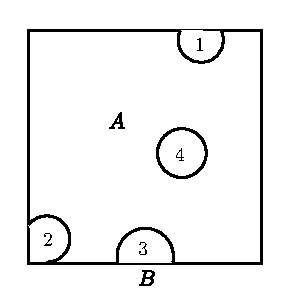
\includegraphics{figure/fig23.eps}
\end{figure}

We will show that $\tau_{i}\subset \overline{\p}(\mathscr{S}_{i}|\mathscr{Z})$ is impossible in each case.

By A.2 in cases (2) and (3) $Lk(\tau_{i},\mathscr{Z})$ is obtained from $Lk(\tau_{i},\mathscr{S})$ by perforations and regular collapses of dimension $(n-\dim\tau_{i}-1)$. In cases (1) and (4) $Lk(\tau_{i},\{\overline{\Delta}_{\tau_{i}}\})$ (with the notation of A.2) is obtained from $Lk(\tau_{i},\mathscr{S})$ by perforations and regular collapses of dimension $(n-\dim\tau_{i}-1)$. By A.3 and remarks thereafter, there cannot be any perforations in cases (1) and (2) and there is exactly one perforation in cases (3) and (4).

By A.1; (b) in the collapse at outer edge $\sigma_{i}$ and major simplex $\Delta_{i}=\sigma_{i}\tau_{i}$, what happens to $Lk(\tau_{i},\mathscr{S}_{i})$ is exactly a perforation\pageoriginale of dimension $(n-\dim \tau_{i}-1)$. So straightaway we have $\tau_{i}\subset \p A-B$ or $\tau_{i}\subset \p B$ is impossible.

So, the only possibilities that remain are (3) and (4). Let us consider case (4) first. We claim that if $\tau_{i}\subset \overline{\p}(\mathscr{S}_{i}|\mathscr{Z})$ the one perforation on $Lk(\tau_{i},\mathscr{S})$ is already made. Since $|Lk(\tau_{i},\mathscr{S})|$ is a sphere, any $(n-1)$-simplex of $\mathscr{S}$ having $\tau_{i}$ as a face must be the face of two $n$-simplexes. So $\tau_{i}$ cannot be in $\overline{\p}(\mathscr{S}_{1}|\mathscr{Z})(\mathscr{S}=\mathscr{S}_{1})$. For the same reason, $\tau_{i}$ cannot be in any $\overline{\p}(\mathscr{S}_{j}|\mathscr{Z})$ with $Lk(\tau_{i},\mathscr{S}_{j})=Lk(\tau_{i},\mathscr{S}_{1})$. Thus $\tau_{i}\subset \overline{\p}(\mathscr{S}_{i}|\mathscr{Z})$ implies $Lk(\tau_{i},\mathscr{S}_{i})\neq Lk(\tau_{i},\mathscr{S}_{1})$. Suppose $Lk(\tau_{i},\mathscr{S})$ is changed for the first time in the $k^{\text{th}}_{i}$ collapse, 
$k_{i}<i$, that is $Lk(\tau_{i},\mathscr{S}_{k_{i}})=Lk(\tau_{i},\mathscr{S}_{1})$, but $Lk(\tau_{i},\mathscr{S}_{k_{i}+1})\neq Lk(\tau_{i},\mathscr{S}_{1})$. Since $Lk(\tau_{i},\mathscr{S}_{1})$ is a sphere; this operation from $Lk(\tau_{i},\mathscr{S}_{1})=Lk(\tau_{i},\mathscr{S}_{k_{i}})$ to $Lk(\tau_{i},\mathscr{S}_{k_{i}+1})$ is necessarily a perforation. So the one perforation on $Lk(\tau_{i},\mathscr{S})$ is already made. But in the $i^{\text{th}}$ collapse also what happens to $Lk(\tau_{i},\mathscr{S}_{i})$ is a perforation since $\Delta_{i}=\sigma_{i}\tau_{i}$ (by A.1.b). Since this is impossible $\tau_{i}$ cannot be in $A-\p A$.

Let us consider the remaining possibility (3), $\tau_{i}\subset B-\p B$. $|Lk(\tau_{i},\mathscr{S})|$ is an $i$-cell with boundary $|Lk(\tau_{i},\mathscr{Z})|$. If $\tau_{i}\subset \overline{\p}(\mathscr{S}_{i}|\mathscr{Z})$, we have to show that $\tau_{i}\subset B-\p B$ is also impossible. The case when $\dim \tau_{i}=n-1$ is easily disposed of, since in that case there is no $n$-simplex having $\tau_{i}$ as a face. As in case (4) $\tau_{i}$ is not in $\overline{\p}(\mathscr{S}_{1}|\mathscr{Z})$ and $\tau_{i}$ cannot be in $\overline{\p}(\mathscr{S}_{j}|\mathscr{Z})$ if $Lk(\tau_{i},\mathscr{S}_{1})=Lk(\tau_{i},\mathscr{S}_{j})$.\pageoriginale Again, the first operation on $Lk(\tau_{i},\mathscr{S}_{1})$ has to be a perforation. For, all the outer edges of $Lk(\tau_{i},\mathscr{S}_{1})$ are in $Lk(\tau_{i},\mathscr{Z})$, and a regular collapse of $Lk(\tau_{i},\mathscr{S}_{1})$ removes a part of $Lk(\tau_{i},\mathscr{Z})$. Thus $\tau_{i}\subset\overline{\p}(\mathscr{S}_{i}|\mathscr{Z})$ implies that the one perforation on $Lk(\tau_{i},\mathscr{S}_{1})$ is already done. But then the result of the $i^{\text{th}}$ collapse will be again a perforation on $Lk(\tau_{i},\mathscr{S}_{i})$ by A.1.b) since $\Delta_{i}=\sigma_{i}\tau_{i}$. So this is again impossible.

Thus $\tau_{i}$ cannot be in $\overline{\p}(\mathscr{S}_{i}|\mathscr{Z})$ for any $i$.
\end{proof}
 

\medskip
\noindent
{\bf A.5.}~ With the hypothesis of A.4., $\overline{\p}(\mathscr{S}_{i}|\mathscr{Z})$ is an $(n-1)$-cell with constant boundary $=\p (|\mathscr{Z}|)=\p B$.

\begin{proof}
$\overline{\p}(\mathscr{S}_{1}|\mathscr{Z})$ is an $(n-1)$-cell with boundary $=\p B$. Inductively, assume that $\overline{\p}(\mathscr{S}_{i}|\mathscr{Z})$ is an $(n-1)$-cell with boundary $\p B$. By A.4, $\tau_{i}\not\subset \overline{\p}(\mathscr{S}_{i}|\mathscr{Z})$; in particular it cannot be in $\p B$. Since $\tau_{i}\not\subset \overline{\p}(\mathscr{S}_{i}|\mathscr{Z})$, no simplex of $\mathscr{S}$ having $\tau_{i}$ as a face can be in $\overline{\p}(\mathscr{S}_{i}|\mathscr{Z})$. So $\p \sigma_{i}\ast \overline{\tau}_{i}$ intersects $\overline{\p}(\mathscr{S}_{i}|\mathscr{Z})$ precisely along $\p \sigma_{i}\ast \p \tau_{i}$. Define $\p_{i}:\overline{\p}(\mathscr{S}_{i}|\mathscr{Z})\to \overline{\p}(\mathscr{S}_{i+1}|\mathscr{Z})$ by $\varphi_{i}$: Identity outside $\overline{\sigma}_{i}\ast \p \tau_{i}$, and on $\overline{\sigma}_{i}\ast \p \tau_{i}$, $\varphi_{i}$ is the join of the identity map on 
$\p \sigma_{i}\ast \p \tau_{i}$ and the map which carries the centre of $\sigma_{i}$ to the centre of $\tau_{i}\cdot \varphi_{i}$ is clearly a polyhedral equivalence; hence $\overline{\p}(\mathscr{S}_{i+1}|\mathscr{Z})$ is an $(n-1)$-cell. To see that $\p(\overline{\p}(\mathscr{S}_{i}|\mathscr{Z}))=\p (\overline{\p}(\mathscr{S}_{i+1}|\mathscr{Z}))$, observe that the part of $\overline{\sigma}_{i}\ast\p\tau_{i}$ (if any) which is in $\p(\overline{\p}(\mathscr{S}_{i}|\mathscr{Z}))$ should be in $\p \sigma_{i}\ast \p \tau_{i}$. Since $\varphi_{i}$ is identity on this part, both the cells have the same boundaries.
\end{proof}



